\documentclass{lab}

\begin{document}

\begin{titlepage}

\pagestyle{empty}	% Нумерация выкл.

\begin{center}
	\textsc{\LARGE Московский Физико-Технический Институт}\\[1,5cm]
	\textsc{\Large Кафедра общей физики}\\[0,5cm]
	\textsc{\large Лабораторная работа \textnumero 3.4.2}\\[2.5cm]

	\noindent\rule{\textwidth}{1pt}
	\\[0.5cm]
	{ \huge \bfseries Закон Кюри-Вейсса}
	\\[0.1cm]
	\noindent\rule{\textwidth}{1pt}
\end{center}

\vfill

\begin{minipage}[b]{0.3\textwidth}
	Маршрут \RomanNumeralCaps{3}\\\\
	20 октября 2018 г.\\
	27 октября 2018 г.
\end{minipage}
\hfill
\begin{minipage}[b]{0.33\textwidth}
	\textit{Работу выполнил}\\
	Ринат Валиев, 711 гр.\\\\
	\textit{Под руководством}\\
	Г.И. Лапушкина, к.ф.-м.н.
\end{minipage}

\end{titlepage}

\pagestyle{VR}
\setcounter{page}{2}

\section*{Подготовка к работе}

\subsection*{Цель работы}

Исследование вынужденных колебаний и процессов их установления.
В работе используются: генератор звуковой частоты, осциллограф, вольтметр, частотометр, ёмкость, индуктивность, магазин сопротивлений, универсальный мост.

\subsection*{Теоретическая часть}

В данной работе будем рассматривать колебания в электрическом колебательном контуре под воздействием внешней ЭДС, гармонически изменяющейся во времени. 
Получаем, что при подключении внешнего источника возникнут колебания, которые будем рассматривать как решение дифференциального уравнения:
\begin{equation}
L\ddot{I} + R \dot{I} + \dfrac{I}{C} = - \mathscr{E} \Omega \sin \Omega t,
\end{equation}
в качестве суперпозиции двух синусоид:
\begin{equation}
I = Be^{-\gamma t} \sin (wt-\theta) + \dfrac{\mathscr{E} \Omega}{L \rho_0} \sin (\Omega t - \psi),
\end{equation}
одна из которых с частотой собственных колебаний контура $\omega$ и амплитудой, экспоненциально убывающей со временем; вторая - с частотой внешнего источника и постоянной амплитудой. Однако со временем собственные колебания затухают, и в контуре устанавливаются вынужденные колебания. А их амплитуда максимальна, когда знаменатель второй синусоиды $\rho_0 = \sqrt{(\omega_0^2 - \Omega^2_0)^2 + (2\gamma \Omega)^2}$ минимален, то есть $\omega_0 = \Omega$ (частота внешнего сигнала совпадает с собственной частотой контура). Это явление и называется \textit{резонансом}. Зависимость амплитуды колебаний от частоты внешнего напряжения называется \textit{резонансной кривой}.

\subsection*{Резонансная кривая колебательного контура}

\begin{wrapfigure}[10]{l}{6cm}
	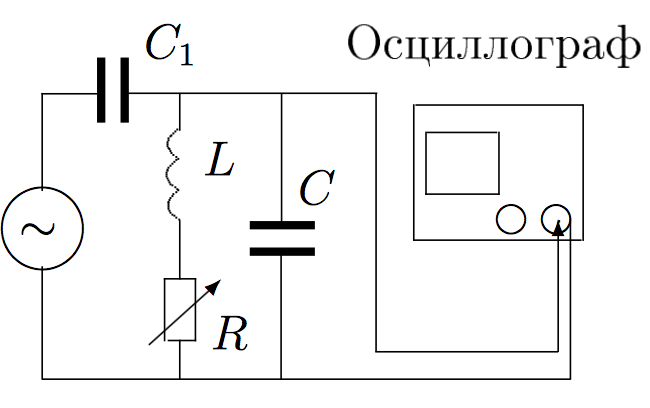
\includegraphics[width=5cm]{Scheme2}
	\caption{\footnotesize Схема установки}
	\label{scheme1}
\end{wrapfigure}

Мы можем снять зависимость амплитуды напряжения на резисторе $R$ от частоты на генераторе (при постоянной амплитуде выходного напряжения), однако для этого выходное сопротивление генератора должно быть много меньше импеданса контура. Для этого в цепи используется конденсатор $C_1$. И в таком случае импеданс внешней по отношению к контуру цепи был гораздо больше импеданса самого контура вблизи резонанса:

$$\dfrac{1}{\omega C_1} \gg |Z_\text{рез}| = \dfrac{L}{RC} $$

\newpage

\subsection*{Процессы установления и затухания колебаний}

\begin{wrapfigure}[12]{l}{7cm}
	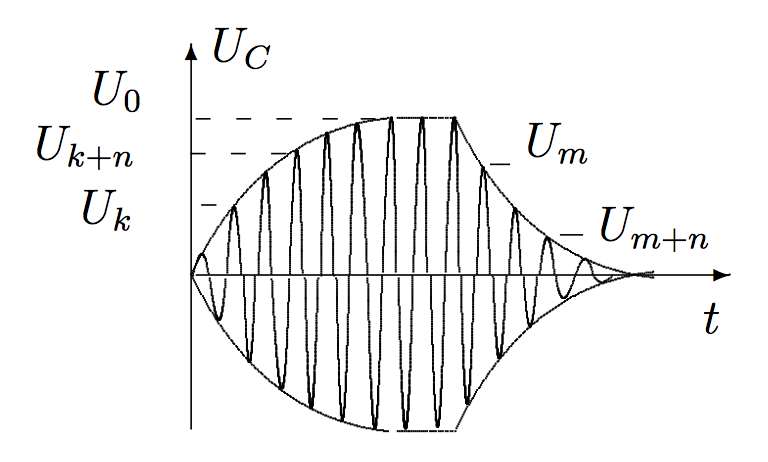
\includegraphics[width=7cm]{Scheme3}
	\caption{\footnotesize Нарастание и затухание вынужденных колебаний}
\end{wrapfigure} 

Добротность контура можно определить и другими способами, например, по скорости затухания свободных колебаний. Подавая на контур цуги синусоид конечной длины, можно наблюдать процессы установления и затухания колебаний в контуре. И те, и другие могут быть использованы для определения добротности контура по скорости нарастания/затухания напряжения:\\

$$\Theta = \dfrac{1}{n} \ln \dfrac{U_0 - U_k}{U_0-U_{k+n}} $$

Измеряя амплитуды напряжения в какой-нибудь момент времени и через n периодов, можем посчитать добротность по формуле:
$$Q = \dfrac{\pi}{\gamma T} = \dfrac{\pi}{\Theta}$$

\section*{Установка и измерения}

\begin{figure}[!h]
	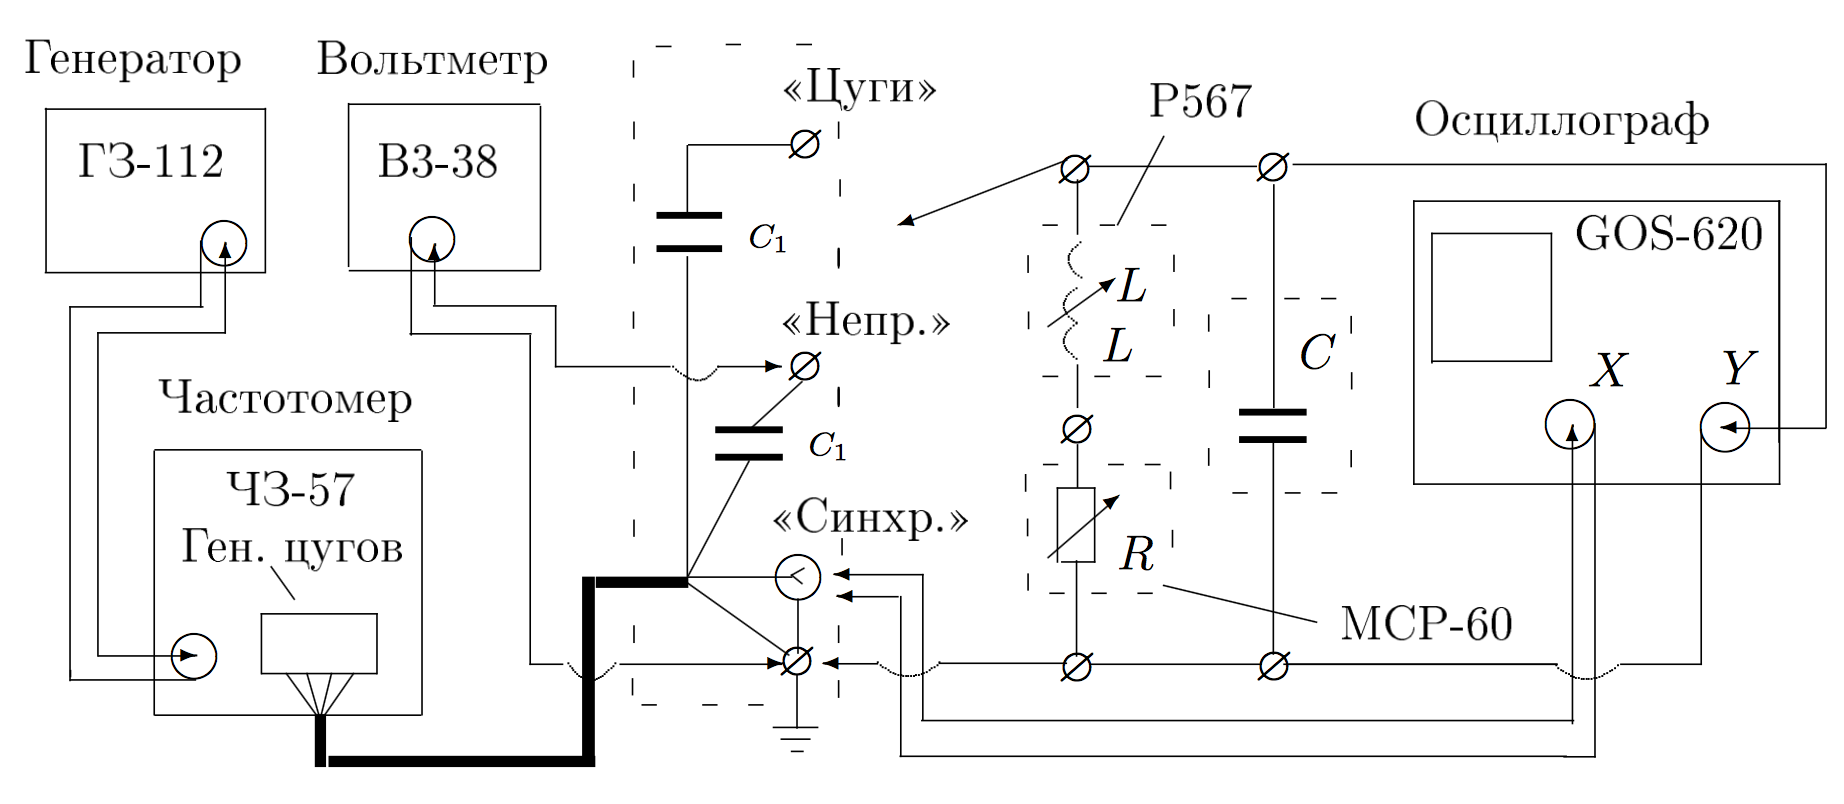
\includegraphics[width = 0.9 \textwidth]{Scheme}
	\caption{\footnotesize Схема экспериментальной установки для исследования вынужденных колебаний}
\end{figure}

Идеальная схема, изображённая на рисунке \ref{scheme1}, не соответствует действительности. Элементы цепи не идеальны и имеют паразитные сопротивления. Измерим все величины для разных частот с помощью RLC – моста:

$$R_L = 22.2 \; \text{Ом},\; L = 99.97 \; \text{мГн}, \; C = 103.33 \; \text{нФ}, \; R = 113.7 \; \text{Ом}$$

\subsection*{Метод резонансных кривых}

Снимем зависимость напряжения на конденсаторе от входной частоты, и получим таким образом резонансную кривую. Также в таблицу внесем погрешности измерений:

\begin{table}[H]
\centering
\renewcommand{\arraystretch}{1.3}
\resizebox{\textwidth}{!}{
	\begin{tabular}{|c|ccccccccccccccc|}
		\hline %\\[-1em]
		$ U $, мВ	&	216	&	332	&	475	&	617	&	775	&	949	&	1139	&	1329	&	1139	&	949	&	760	&	617	&	443	&	316	&	240	\\ \hline %\\[-1em]
		$ f $, кГц	&	1,442	&	1,478	&	1,504	&	1,518	&	1,528	&	1,539	&	1,548	&	1,561	&	1,574	&	1,582	&	1,594	&	1,608	&	1,630	&	1,661	&	1,700	\\ \hline %\\[-1em]
		$ U/U_0 $	&	0,163	&	0,250	&	0,357	&	0,464	&	0,583	&	0,714	&	0,857	&	1,000	&	0,857	&	0,714	&	0,572	&	0,464	&	0,333	&	0,238	&	0,181	\\ \hline %\\[-1em]
		$ f/f_0 $	&	0,921	&	0,944	&	0,960	&	0,969	&	0,976	&	0,983	&	0,989	&	0,997	&	1,005	&	1,010	&	1,018	&	1,027	&	1,041	&	1,061	&	1,086	\\ \hline %\\[-1em]
		$ \Delta \; {U}/{U_0} $	&	0,002	&	0,002	&	0,002	&	0,002	&	0,002	&	0,003	&	0,003	&	0,003	&	0,003	&	0,003	&	0,002	&	0,002	&	0,002	&	0,002	&	0,002	\\ \hline %\\[-1em]
		$ \Delta \; f/f_0 $	&	0,002	&	0,002	&	0,003	&	0,003	&	0,003	&	0,003	&	0,003	&	0,003	&	0,003	&	0,003	&	0,003	&	0,003	&	0,003	&	0,003	&	0,003	\\ \hline
	\end{tabular}}
\renewcommand{\arraystretch}{1}
\caption{\footnotesize Полученные значения при R = 0 Ом}
\label{tab1}
\end{table}

\begin{table}[H]
\centering
\renewcommand{\arraystretch}{1.3}
\resizebox{\textwidth}{!}{
\begin{tabular}{|c|cccccccccccccc|}
		\hline
		$ U $, мВ	&	78	&	94	&	108	&	138	&	182	&	246	&	282	&	264	&	228	&	192	&	153	&	126	&	96	&	82	\\ \hline
		$ f $, кГц	&	1,276	&	1,316	&	1,360	&	1,410	&	1,460	&	1,511	&	1,564	&	1,608	&	1,652	&	1,694	&	1,762	&	1,831	&	1,955	&	2,172	\\ \hline
		$ U/U_0 $	&	0,277	&	0,333	&	0,383	&	0,489	&	0,645	&	0,872	&	1,000	&	0,936	&	0,809	&	0,681	&	0,543	&	0,447	&	0,340	&	0,291	\\ \hline
		$ f/f_0 $	&	0,815	&	0,840	&	0,868	&	0,900	&	0,932	&	0,965	&	0,999	&	1,027	&	1,055	&	1,082	&	1,125	&	1,169	&	1,248	&	1,387	\\ \hline
		$ \Delta \; {U}/{U_0} $	&	0,001	&	0,001	&	0,001	&	0,001	&	0,001	&	0,001	&	0,001	&	0,001	&	0,001	&	0,001	&	0,001	&	0,001	&	0,001	&	0,001	\\ \hline
		$ \Delta \; f/f_0 $	&	0,002	&	0,002	&	0,002	&	0,002	&	0,002	&	0,003	&	0,003	&	0,003	&	0,003	&	0,003	&	0,003	&	0,003	&	0,003	&	0,003	\\ \hline
\end{tabular}}
\renewcommand{\arraystretch}{1}
\caption{\footnotesize Полученные значения при R = 100 Ом}
\label{tab2}
\end{table}

Используя полученные данные построим резонансные кривые для каждой величины сопротивления:

\begin{figure}[H]
	\centering
	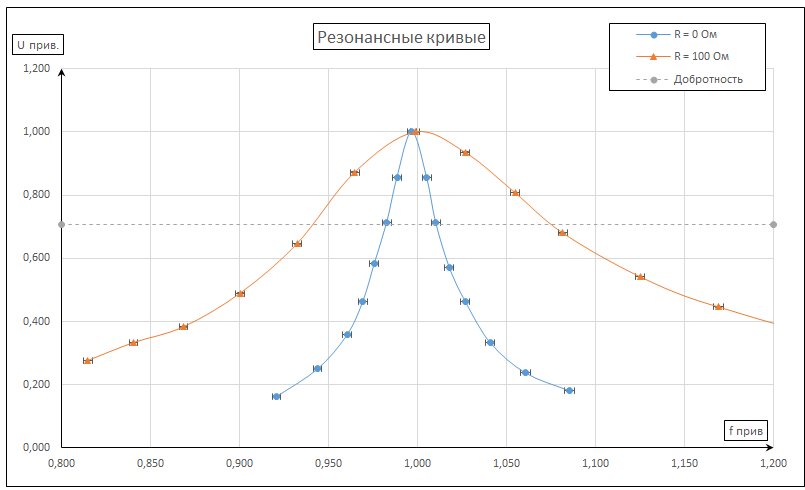
\includegraphics[width = 0.9 \textwidth]{Graph}
	\caption{\footnotesize Резонансные кривые для $R = 0$ Ом, $R = 1000$ Ом в приведенных координатах}
\end{figure}

\newpage

\subsection*{Метод цугов}

Добротность можно определить и другим способ. Будем посылать на осциллограф синусоидальный сигнал порциями. Тогда на экране увидим как сигнал нарастает и затухает. В условиях резонанса огибающая затухающих колебаний -- это перевернутая огибающая нарастающего участка.
Снимем три пары точек для дальнейших вычислений:

\begin{table}[H]
	\centering
	\renewcommand{\arraystretch}{1.3}
	\begin{tabular}{|c|c|c|c|c|c|c|c|c|c|c|c|c|}
		\hline
		& \multicolumn{6}{c|}{Нарастание} & \multicolumn{6}{c|}{Затухание} \\ \hline
		$R$, Ом & \multicolumn{3}{c|}{0} & \multicolumn{3}{c|}{100} & \multicolumn{3}{c|}{0} & \multicolumn{3}{c|}{100} \\ \hline
		$U_{0}$, дел & \multicolumn{3}{c|}{39} & \multicolumn{3}{c|}{40} & \multicolumn{6}{c|}{-} \\ \hline
		$U_{k}$, дел & 4 & 7 & 10 & 10 & 20 & 10 & 37 & 36 & 32 &40 & 31.5 & 40 \\ \hline
		$U_{k+n}$, дел & 24.5 & 30 & 35 & 37.5 & 37.5 & 36 & 16.5 & 10 & 5 & 4 & 4 & 6.5\\ \hline
		n & 9 & 13 & 20 & 6 & 5 & 5 & 9 & 13 & 20 & 6 & 5 & 5\\ \hline
		Q & 32.1 & 32.2 & 31.7 & 7.6 & 7.6 & 7.8 & 35.0 & 31.9 & 33.8 & 8.2 & 7.6 & 8.6\\ \hline
	\end{tabular}
	\caption{\footnotesize Измерение добротности по нарастанию и затуханию}
	\label{tab3}
	\renewcommand{\arraystretch}{1}
\end{table}

Используем данные таблицы \ref{tab3} и формулы в начале работы для расчета добротности по скорости нарастания и затухания колебаний. Результаты внесем в таблицу \ref{tab4}.

\subsection*{Погрешности}

Погрешности измерений и вычислений определим через параметры приборов и по шкале осциллографа. Приведем лишь некоторые формулы расчета погрешностей:

Для погрешности теоретического вычисления погрешности используем:

\begin{equation}
\begin{aligned}
	&\Delta_Q = \sqrt{\left( \dfrac{\partial Q}{\partial R} \right)^2 \cdot \Delta_R^2 + \left( \dfrac{\partial Q}{\partial L} \right)^2 \cdot \Delta_L^2 + \left( \dfrac{\partial Q}{\partial C} \right)^2 \cdot \Delta_C^2} \\
	&\Delta_Q = \sqrt{\dfrac{L}{R^4C} \cdot \Delta_R^2 + \dfrac{1}{4R^2LC} \cdot \Delta_L^2 + \dfrac{L}{4C^3R^2} \cdot \Delta_C^2}
\end{aligned}
\end{equation}

В случае вычисления добротности через затухающую часть графика имеем:

\begin{equation}
\begin{aligned}
	&Q = \dfrac{\pi}{\Theta} , ~~~ где \ \Theta = \frac{1}{n} \ln (\dfrac{U_k}{U_{k+n}})\\
	&\Delta_{\Theta} = \sqrt{\left( \dfrac{\partial {\Theta}}{\partial U_k} \right)^2 \cdot \Delta_{U_k}^2 + \left( \dfrac{\partial {\Theta}}{\partial U_{k+n}} \right)^2 \cdot \Delta_{U_{k+n}}^2}\\
	&\Delta_Q = \pi \cdot \frac{\Delta_{\Theta}}{\Theta^2}
\end{aligned}
\end{equation}

\section*{Итоги}

В работе были определены добротности контуров с и без дополнительного сопротивления
$ R_{100} $ разными способами.

\begin{table}[H]
	\centering
	\renewcommand{\arraystretch}{1.3}
	\begin{tabular}{|c|c|c|c|c|}
		\hline
		& Теория & Резонансная кривая & Нарастание & Убывание     \\ \hline
		$Q_{R=0}$   & 36.2   & $34.5 \pm 1.2$     & $32 \pm 4$ & $33.6 \pm 3$ \\ \hline
		$Q_{R=100}$ & 7.0   & $6.2 \pm 0.4$      & $7.6 \pm 1$  & $8.1 \pm 1$  \\ \hline
	\end{tabular}
	\caption{\footnotesize Сравнение экспериментальных значений добротности, полученных разными методами}
	\label{tab4}
	\renewcommand{\arraystretch}{1}
\end{table}

В целом добротности оказались примерно одинаковыми при измерении разными способами. Однако, результаты немного разнятся. Следует заметить, что магазин сопротивлений мог дать значительный вклад для сопротивления в контуре с $ R = 0 $ Ом, т.к. резисторы собраны в виде катушек. Данный факт не был учтен в работе.

\subsubsection*{Замечание}
Рассмотрим процесс установления колебаний в контуре с высокой добротностью вблизи резонанса.
Этот процесс описывается при начальных условиях $ (U = 0, \ddot{U} = 0) $ формулой:
$$ U = U_0[\cos(\Omega t - \psi) - \exp^{\gamma t} \cos (\omega_0 t - \psi)] $$
Напряжение содержит два близких по частоте колебания, между которыми происходят биения. Появление биений связано с тем, что разность фаз этих колебаний медленно меняется; при нулевой разности фаз они вычитаются друг из друга, а при расхождении фаз на $ \pi $ -- складываются. Амплитуда колебаний то растет, то падает, испытывая биения. При порционных сигналах также наблюдаются схожая картина.

\begin{figure}[!h]
	\centering
	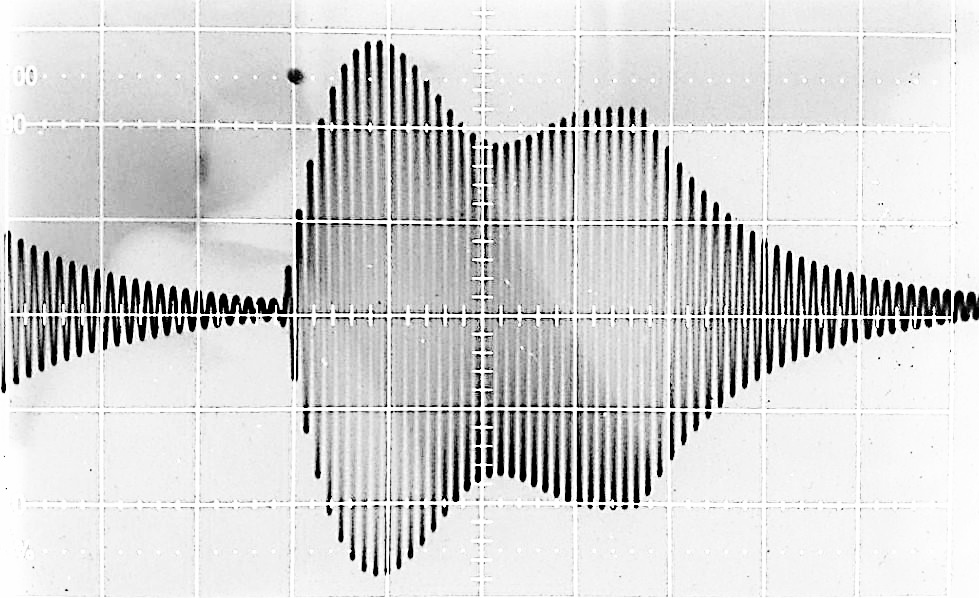
\includegraphics[width = 0.5 \textwidth]{cool}
	\caption{\footnotesize Биение колебаний вблизи резонанса}
\end{figure}

\end{document}